\documentclass[a4paper,10pt]{article}
\usepackage{amsmath}
\usepackage[italian]{babel}
\usepackage[utf8]{inputenc}
\usepackage{graphicx}

\begin{document}

\title{Report - Primo assegnamento Ingegneria del Software}
\author{Vincenzo Arceri - VR360465\\
 Matteo Calabria - VR363871\\
 Pietro Musoni - VR359914\\ 
Carlo Tacchella - VR362194\\}
\date{Anno accademico 2013/2014}
\maketitle

\section{Specifiche del progetto}

Il \textit{Car Park System} è un esempio di sistema embedded distribuito che usa reti e dispositivi elettronici.
Principalmente, il sistema è composto da nodi e canali di comunicazione. I nodi possono essere sensori, unità aritmetiche,
router, display, etc...  I canali possono essere wireless o cablati.
Il car park system mostra il numero medio di macchine all'ora e il numero di posti disponibili. 
Lo scenario di applicazione è:
\begin{itemize}
\item il \textit{car detector} rileva l'ingresso e l'uscita delle automobili e manda un messaggio alla processing unit;
\item la \textit{processing unit} calcola la nuova media oraria di automobili entrate e manda il risultato al monitor;
\item la processing unit calcola il numero di posti disponibili rimanenti sottraendo il numero di auto entrate dalla capacità massima del parcheggio (assumiamo che la capacità del parcheggio sia di 500 automobili).
\end{itemize}
Tutti questi messaggi sono scambiati su un unico canale wireless.

\section{Scelte progettuali}
Il diagramma delle classi riporta il prototipo del progetto, mostrando graficamente le scelte implementative, le assunzioni ed i pattern utilizzi (Figura 1). I differenti canali di comunicazione sono espressi da tre interfacce, che estendono tutte un'interfaccia \textit{marker} \textbf{NodeCommunication}:  \textbf{TxCommunication}, interfaccia implementata esclusivamente dai nodi trasmettitori, \textbf{RxCommunication}, interfaccia implementata escluviamente dai nodi ricevitori e \textbf{TxRxCommunication} è l'interfaccia implementata dai nodi che trasmettono e ricevono dati. L'interfaccia di trasmissione ha quattro metodi, \textit{send} e \textit{set}, che rispettivamente mandano il dato sul canale di trasmissione e preparano il dato per poter essere spedito successivamente, \textit{registerObserver} e \textit{unregisterObserver} che sono metodi tipici del pattern di progettazione utilizzato, di cui parlermo ampiamente nella sezione successiva; l'interfaccia di ricezione implementa i metodi speculari, \textit{receive} e \textit{read}, che rispettivamente riceve un dato e lo legge, rendendolo effettivamente utilizzabile (nel nostro caso per successive computazioni e per mostrare il risultato della computazione nei diversi display).

\begin{figure}[htbp]
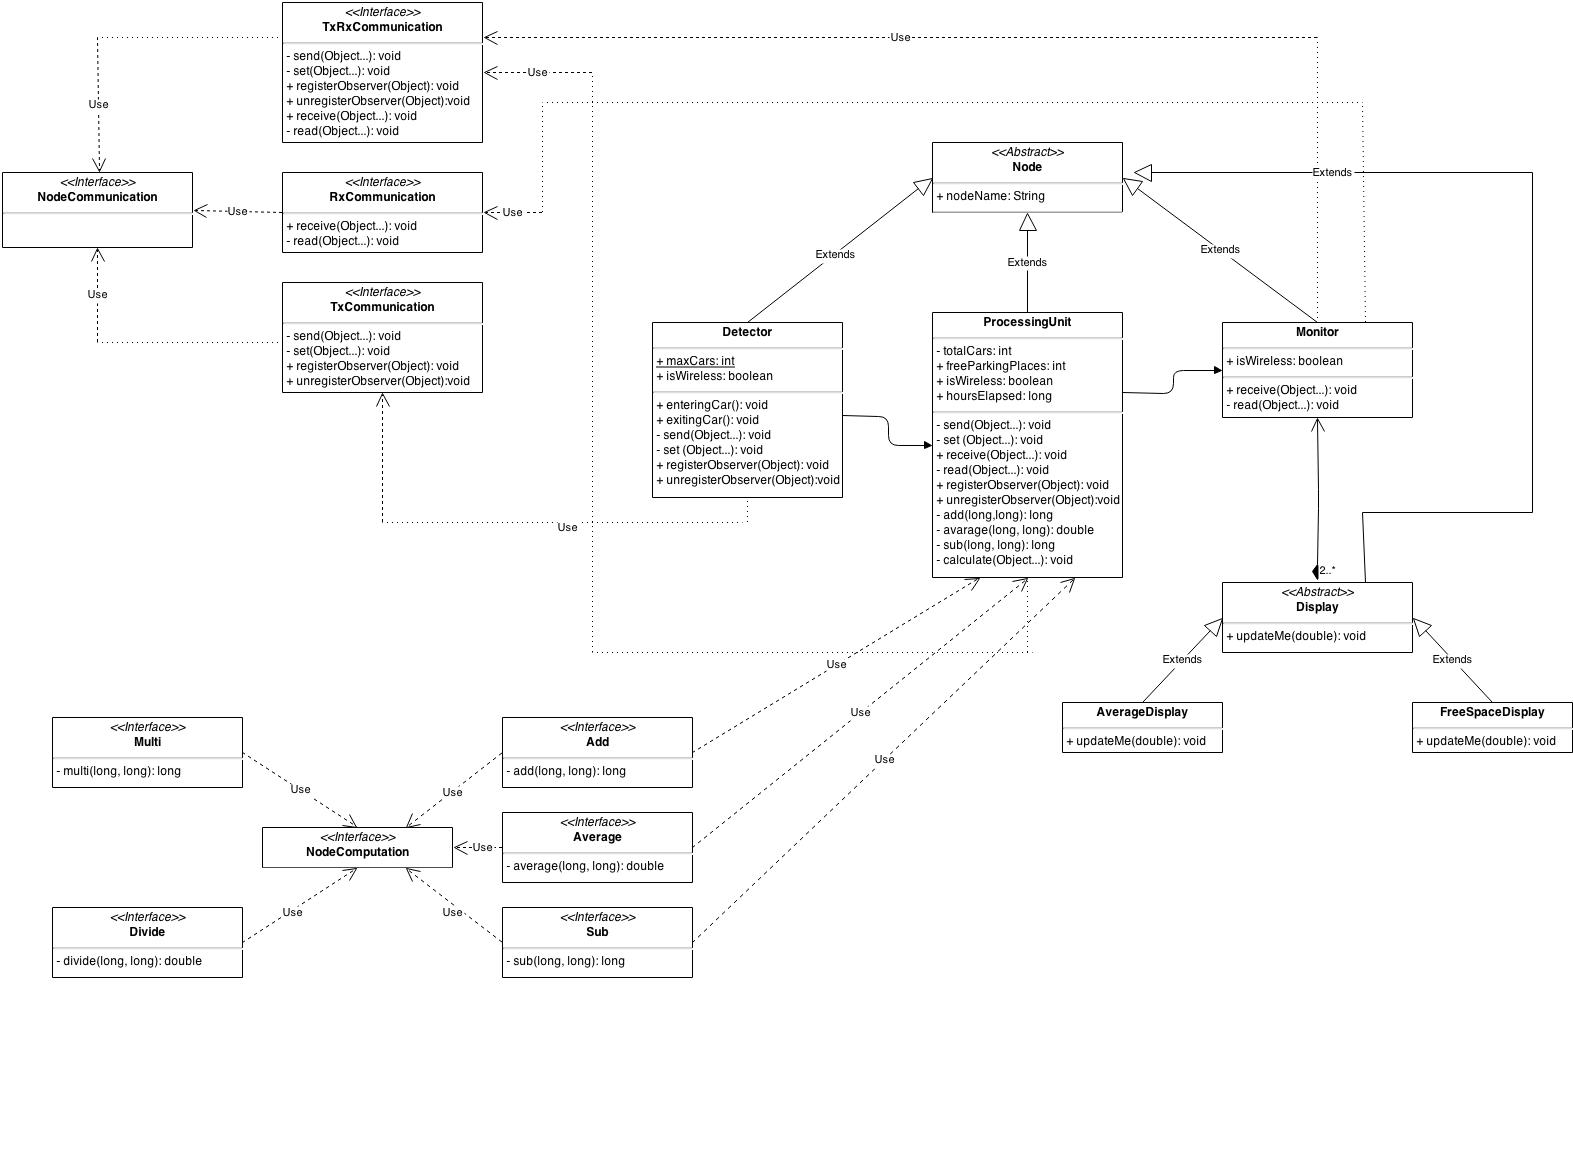
\includegraphics[scale=0.24]{class_diagram.jpg}
\caption{Diagramma delle classi}
\label{class_dig}
\end{figure}

Ogni nodo estende un'interfaccia marker \textbf{Node}, al cui interno c'è un campo \textit{nodeName} che identifica un nodo. I nodi in questa prima versione del software sono tre: 
\begin{itemize}
\item \textbf{Detector}: è il primo nodo ad essere attivato nel più comune degli scenari, cioè quando entra o esce una macchina; il suo compito è quello di segnalare l'entrata o l'uscita di una macchina alla ProcessingUnit;
\item \textbf{ProcessingUnit}: è il nodo adibito alla computazione; riceve dati da Detector, li elabora calcolando la nuova media e i posti macchina liberi, inviando i dati al Monitor;
\item \textbf{Monitor}: per quanto riguarda questo nodo, abbiamo assunto che sia composto da diversi display, uno per ogni dato che si vuole mostrare: secondo noi è la scelta più funzionale in vista di possibili estensioni e in accordo con i principi base della programmazione ad oggetti e dell'ingegneria del software.
\end{itemize}

Il Monitor è composto da diversi Display, che estendono a loro volta la classe astratta \textit{Node}; in questa prima versione del software i display sono solamente due, \textit{AverageDisplay} e \textit{FreeParksDisplay}, come richiesto dalle specifiche; in questo modo, se in futuro ci fosse la necessità di aggiungere nuovi display, è possibile farlo semplicemente estendendo la classe \textit{Display} ed aggiungere il nuovo componente al Monitor.

Infine, la maggior parte dei metodi implementati richiedono come parametro un \textit{Object} o una sua lista: tale scelta implementativa è stata fatta per garantire la possibilità di passare come parametro più oggetti di diverso tipo, senza stravolgere l'architettura di base: saranno poi le singole classi ad implementare la specifica versione di quel metodo, effettuando opportuni controlli di tipo.

La media, nella nostra simulazione, rappresenta il numero medio orario di veicoli entrati da quando il sistema è attivo: l'utente può aumentare le ore trascorse da quando il sistema è attivo (di default il sistema è funzionante da un'ora). 
Il numero massimo di posti auto è memorizzato nella variabile statica \textit{maxCars}, presente nella classe Detector: dato che ogni controllo sulle postazioni viene fatto tramite questa variabile è possibile adattare questo software a parcheggi con capienze differenti.

La classe Simulator contiene un main per la simulazione grafica ed il setup del sistema: sarà appunto tale main a creare i nodi ed a registrarli agli opportuni oggetti. Tramite l'interfaccia utente è possibile simulare l'entrate e l'uscita di un veicolo ed aumentare le ore su cui la media deve essere calcolata. Di seguito è mostrato uno screenshot dell'applicazione.

\begin{figure}[htbp]
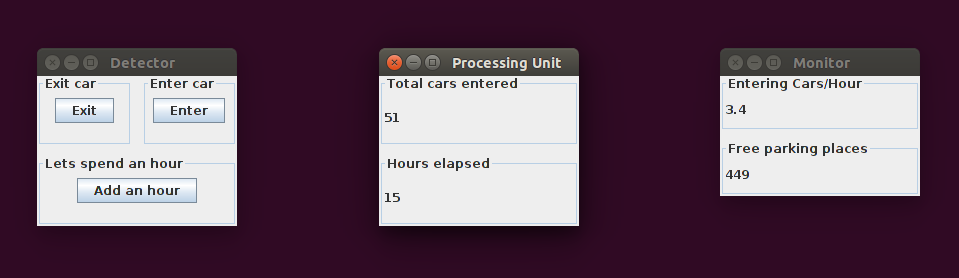
\includegraphics[scale=0.4]{screenshot.png}
\caption{Screenshot dell'applicazione}
\label{class_dig}
\end{figure}

\section{Design pattern utilizzati}
Il principale design pattern applicato è il pattern \textit{Observer}, che spieghiamo nei due casi di seguito.   

Il primo scenario in cui viene applicato è tra Detector e ProcessingUnit: nello stato di setup del sistema, automaticamente l'oggetto ProcessingUnit, che ricopre il ruolo di Observer, si registrerà presso il Detector, che invece svolge il ruolo di Subject; nel momento in cui entra o esce un veicolo il Detector chiamerà il metodo \textit{set} per prepare il dato e successivamente inviarlo tramite il metodo \textit{send}: quest'ultimo invoceherà automaticamente il metodo pubblico \textit{receive}, che funge da metodo di notifica tipico del pattern in questione.

Il secondo caso è quello tra ProcessingUnit, che questa volta ricopre il ruolo di Subject, e Monitor, che svolge il ruolo di Observer: una volta ricevuti i dati dal Detector, la ProcessingUnit ricalcolerà  i posti disponibili e l'eventuale media oraria, invocherà il metodo \textit{set} per preparare il dato e successivamente inviarlo tramite il metodo \textit{send}: questo invocherà il metodo pubblico \textit{receive}, che come prima funge da metodo di notifica tipico del pattern.

Le inferfacce per identificare Subject e Observer sono le stesse interfacce per la comunicazione: RxCommunication viene estesa dagli oggetti Observer, che contiene il metodo \textit{receive} che viene invocato dai Subject, tramite il metodo \textit{send} dell'interfaccia TxCommunication.

Si può notare come una stessa classe, ProcessingUnit, venga utilizzata più volte per uno stesso tipo di pattern, ma con ruoli diversi a seconda del contesto e quindi dell'oggetto con cui si mette in relazione: svolge infatti il ruolo di Observer nei confronti del Detector e il ruolo di Subject nei confronti del Monitor.

Le registrazioni presso i diversi Observer vengono effettuate dalla classe Simulator.

\end{document}